\section{Object-Oriented Modeling and UML Design}
\label{sec:uml_design}

\subsection{Overview of UML Modeling in System Engineering}
The Unified Modeling Language (UML) is the industry-standard visual modeling language used to specify, visualize, construct, and document the artifacts of software-intensive systems \cite{fowler2003uml}. In an Object-Oriented Methodologies curriculum, UML serves as the conceptual blueprint bridging high-level functional requirements and concrete object-oriented source code.

This chapter presents an exhaustive architectural analysis of the Online Auction Management System (BidNexus) across eight standard UML diagram types: Use Case, Class, Sequence (five detailed scenarios), Activity, State Machine, Component, Deployment, and Entity-Relationship. All diagrams were modeled formally in PlantUML and rendered to high-resolution vector/raster graphics directly reflecting the underlying Java implementation.

% ==============================================================================
% 1. USE CASE DIAGRAM
% ==============================================================================
\subsection{Use Case Diagram}
\label{subsec:uml_use_case}

\subsubsection{Diagram Visualization}
Figure \ref{fig:use_case} depicts the high-level functional capabilities exposed to the system's human actors.

\begin{figure}[H]
    \centering
    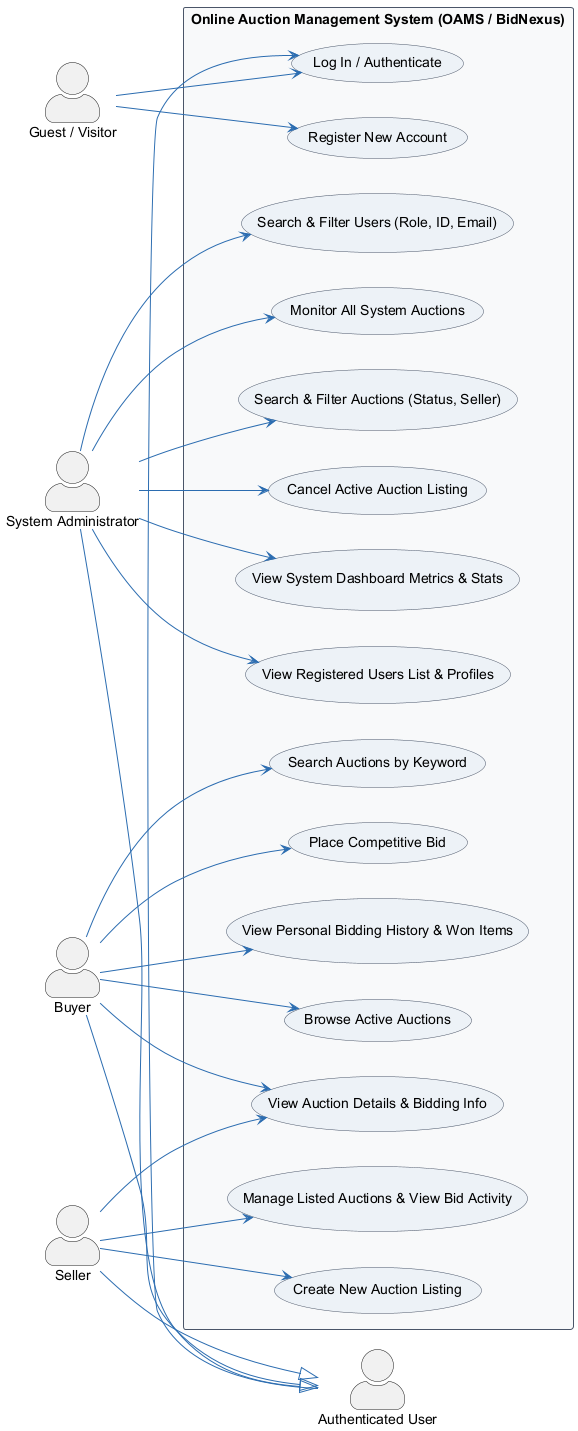
\includegraphics[width=0.95\textwidth]{figures/use_case_diagram.png}
    \caption{UML Use Case Diagram for Online Auction Management System}
    \label{fig:use_case}
\end{figure}

\subsubsection{Structural and Behavioral Analysis}
The Use Case diagram delineates the system boundary of BidNexus and models actor interactions:
\begin{itemize}
    \item \textbf{Actor Hierarchy and Generalization:} An unauthenticated actor begins as a \textit{Guest / Visitor}, restricted to registering an account or initiating login. Upon successful authentication, the actor generalizes into an \textit{Authenticated User}. \textit{Buyer}, \textit{Seller}, and \textit{System Administrator} inherit this authenticated base status while branching into specialized roles.
    \item \textbf{Buyer Domain Use Cases:} Buyers interact with use cases governing catalog exploration and purchase: \textit{Browse Active Auctions}, \textit{Search Auctions by Keyword}, \textit{View Auction Details}, \textit{Place Competitive Bid}, and \textit{View Personal Bidding History \& Won Items}.
    \item \textbf{Seller Domain Use Cases:} Sellers interact with inventory liquidation features: \textit{Create New Auction Listing}, \textit{Manage Listed Auctions}, and \textit{Inspect Received Bids}.
    \item \textbf{Administrator Domain Use Cases:} Privileged operators interact with system governance functions: \textit{View Registered Users List}, \textit{Search \& Filter Users}, \textit{Monitor All System Auctions}, \textit{Filter Auctions by Status}, \textit{Cancel Active Listing}, and \textit{View System Dashboard Metrics}.
\end{itemize}

% ==============================================================================
% 2. CLASS DIAGRAM
% ==============================================================================
\subsection{Class Diagram (Structural Architecture)}
\label{subsec:uml_class}

\subsubsection{Diagram Visualization}
Figure \ref{fig:class_diagram} illustrates the static structural design of BidNexus, detailing classes, attributes, operations, visibility modifiers, and inter-class relationships.

\begin{figure}[H]
    \centering
    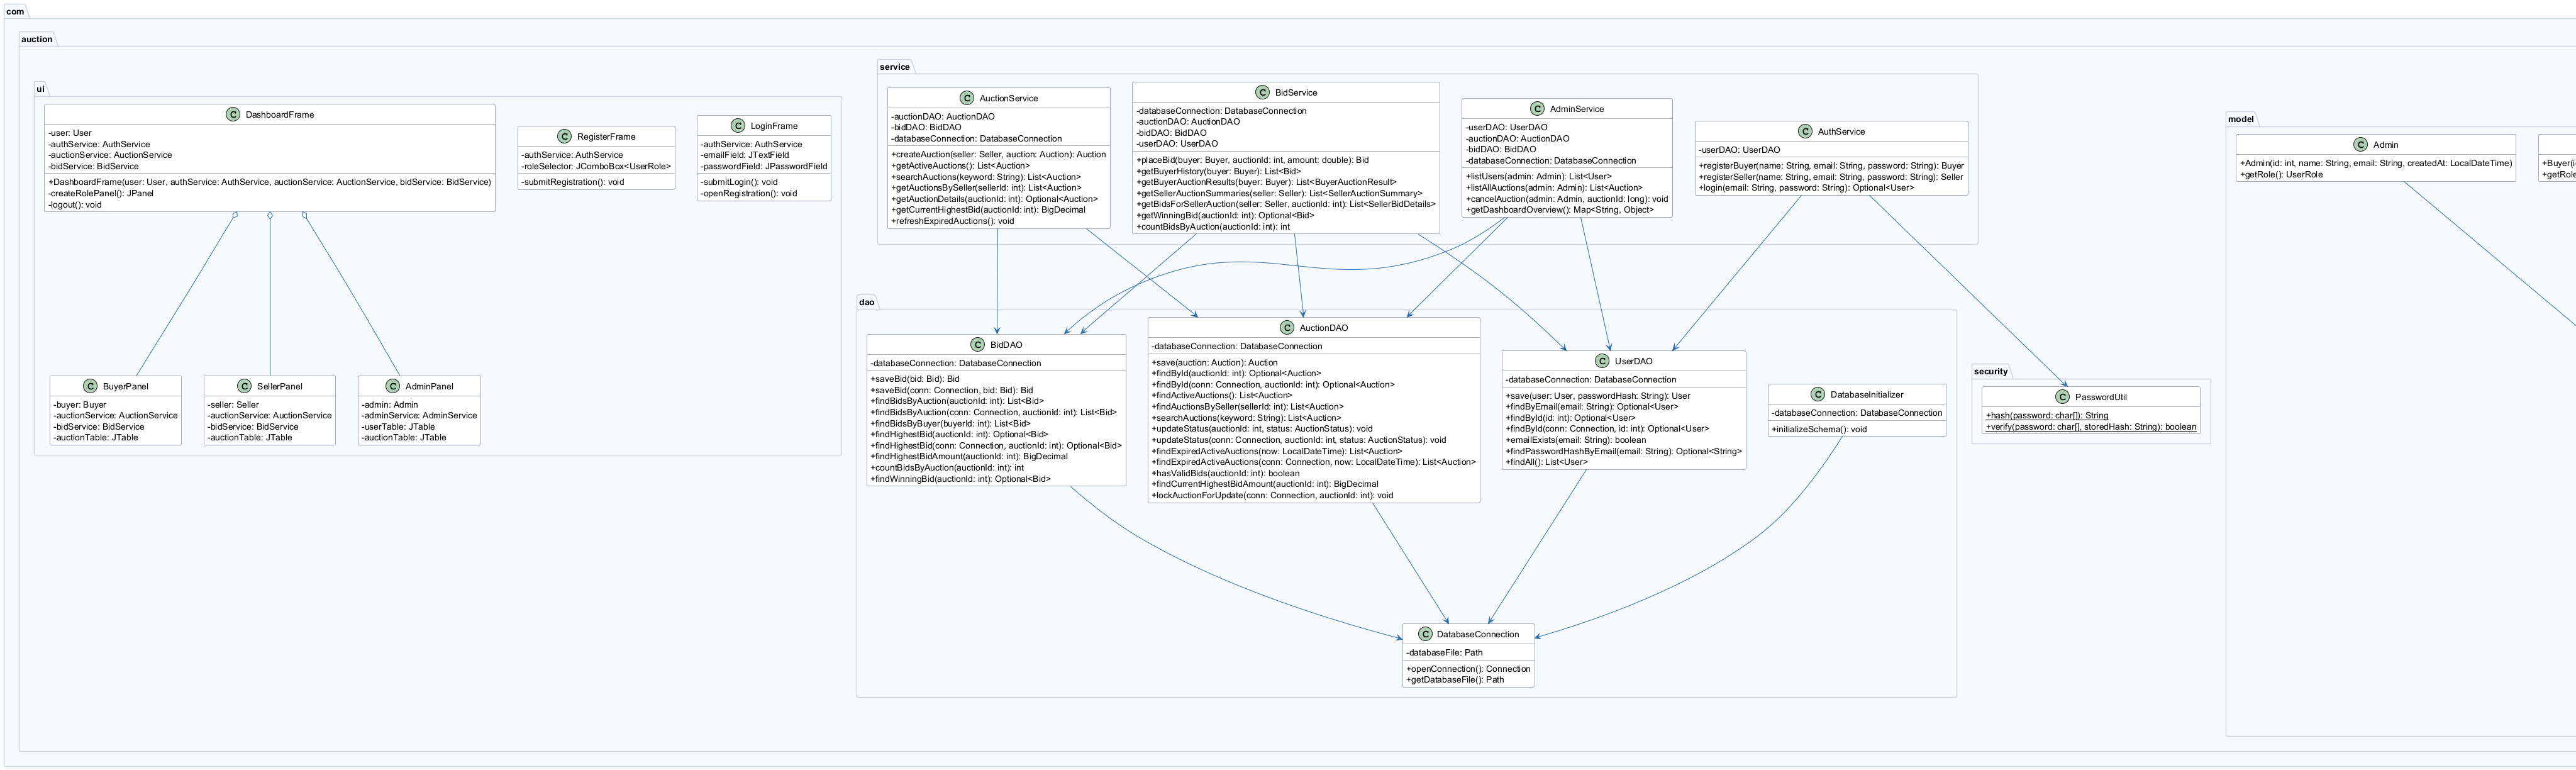
\includegraphics[width=\textwidth]{figures/class_diagram.png}
    \caption{UML Class Diagram Depicting Model, Service, DAO, and GUI Packages}
    \label{fig:class_diagram}
\end{figure}

\subsubsection{Detailed Class and Relationship Walkthrough}
The class structure is organized into five cohesive packages following clean architecture principles \cite{martin2017clean}:

\paragraph{1. Package \texttt{com.auction.model}:}
Houses the domain abstractions and core entities:
\begin{itemize}
    \item \texttt{User} (Abstract Class): Represents common identity state (\texttt{id}, \texttt{name}, \texttt{email}, \texttt{createdAt}). Contains private final fields, constructor validation, and the abstract method \texttt{getRole(): UserRole}.
    \item \texttt{Buyer}, \texttt{Seller}, \texttt{Admin} (Concrete Subclasses): Extend \texttt{User} through inheritance, overriding \texttt{getRole()} to return \texttt{BUYER}, \texttt{SELLER}, and \texttt{ADMIN} respectively.
    \item \texttt{Auction}: Models the auction entity with attributes including \texttt{startingPrice}, \texttt{endTime}, and \texttt{status}. Encapsulates expiration logic via \texttt{isExpired(LocalDateTime)}.
    \item \texttt{Bid}: Represents an immutable monetary bid with \texttt{auctionId}, \texttt{buyerId}, \texttt{amount}, and \texttt{bidTime}.
    \item Enumerations: \texttt{UserRole} (\texttt{BUYER, SELLER, ADMIN}) and \texttt{AuctionStatus} (\texttt{ACTIVE, SOLD, UNSOLD, CANCELLED}).
\end{itemize}

\paragraph{2. Package \texttt{com.auction.service}:}
Contains business logic and policy enforcement:
\begin{itemize}
    \item \texttt{AuthService}: Orchestrates credential checking and user onboarding.
    \item \texttt{AuctionService}: Manages auction creation, catalog queries, keyword search, and lazy expiration sweeping.
    \item \texttt{BidService}: Coordinates transactional bid submission, row-level concurrency locking, self-bid rejection, and winner determination.
    \item \texttt{AdminService}: Provides administrative monitoring aggregations, multi-attribute searches, and safe listing cancellation.
\end{itemize}

\paragraph{3. Package \texttt{com.auction.dao}:}
Implements the Data Access Object pattern:
\begin{itemize}
    \item \texttt{DatabaseConnection}: Manages JDBC connections to SQLite and enforces foreign key support via \texttt{PRAGMA foreign\_keys = ON}.
    \item \texttt{UserDAO}, \texttt{AuctionDAO}, \texttt{BidDAO}: Contain parameterized SQL queries using \texttt{PreparedStatement} to prevent SQL injection and map relational rows to domain objects.
    \item \texttt{DatabaseInitializer}: Executes idempotent DDL schema generation scripts.
\end{itemize}

\paragraph{4. Package \texttt{com.auction.security}:}
Contains \texttt{PasswordUtil}, providing static cryptographic routines for PBKDF2 with HMAC-SHA256 password hashing and salt verification.

\paragraph{5. Package \texttt{com.auction.ui}:}
Implements the desktop user interface using Java Swing. \texttt{DashboardFrame} serves as the primary container, aggregating \texttt{BuyerPanel}, \texttt{SellerPanel}, and \texttt{AdminPanel}.

% ==============================================================================
% 3. SEQUENCE DIAGRAMS
% ==============================================================================
\subsection{Sequence Diagrams (Behavioral Interactions)}
\label{subsec:uml_sequence}

Sequence diagrams model runtime object interactions arranged in temporal sequence, illustrating message passing between UI boundaries, control services, DAOs, and the database engine.

\subsubsection{Scenario A: Buyer Placing a Competitive Bid}
Figure \ref{fig:seq_bid} traces the execution path when a Buyer submits a bid.

\begin{figure}[H]
    \centering
    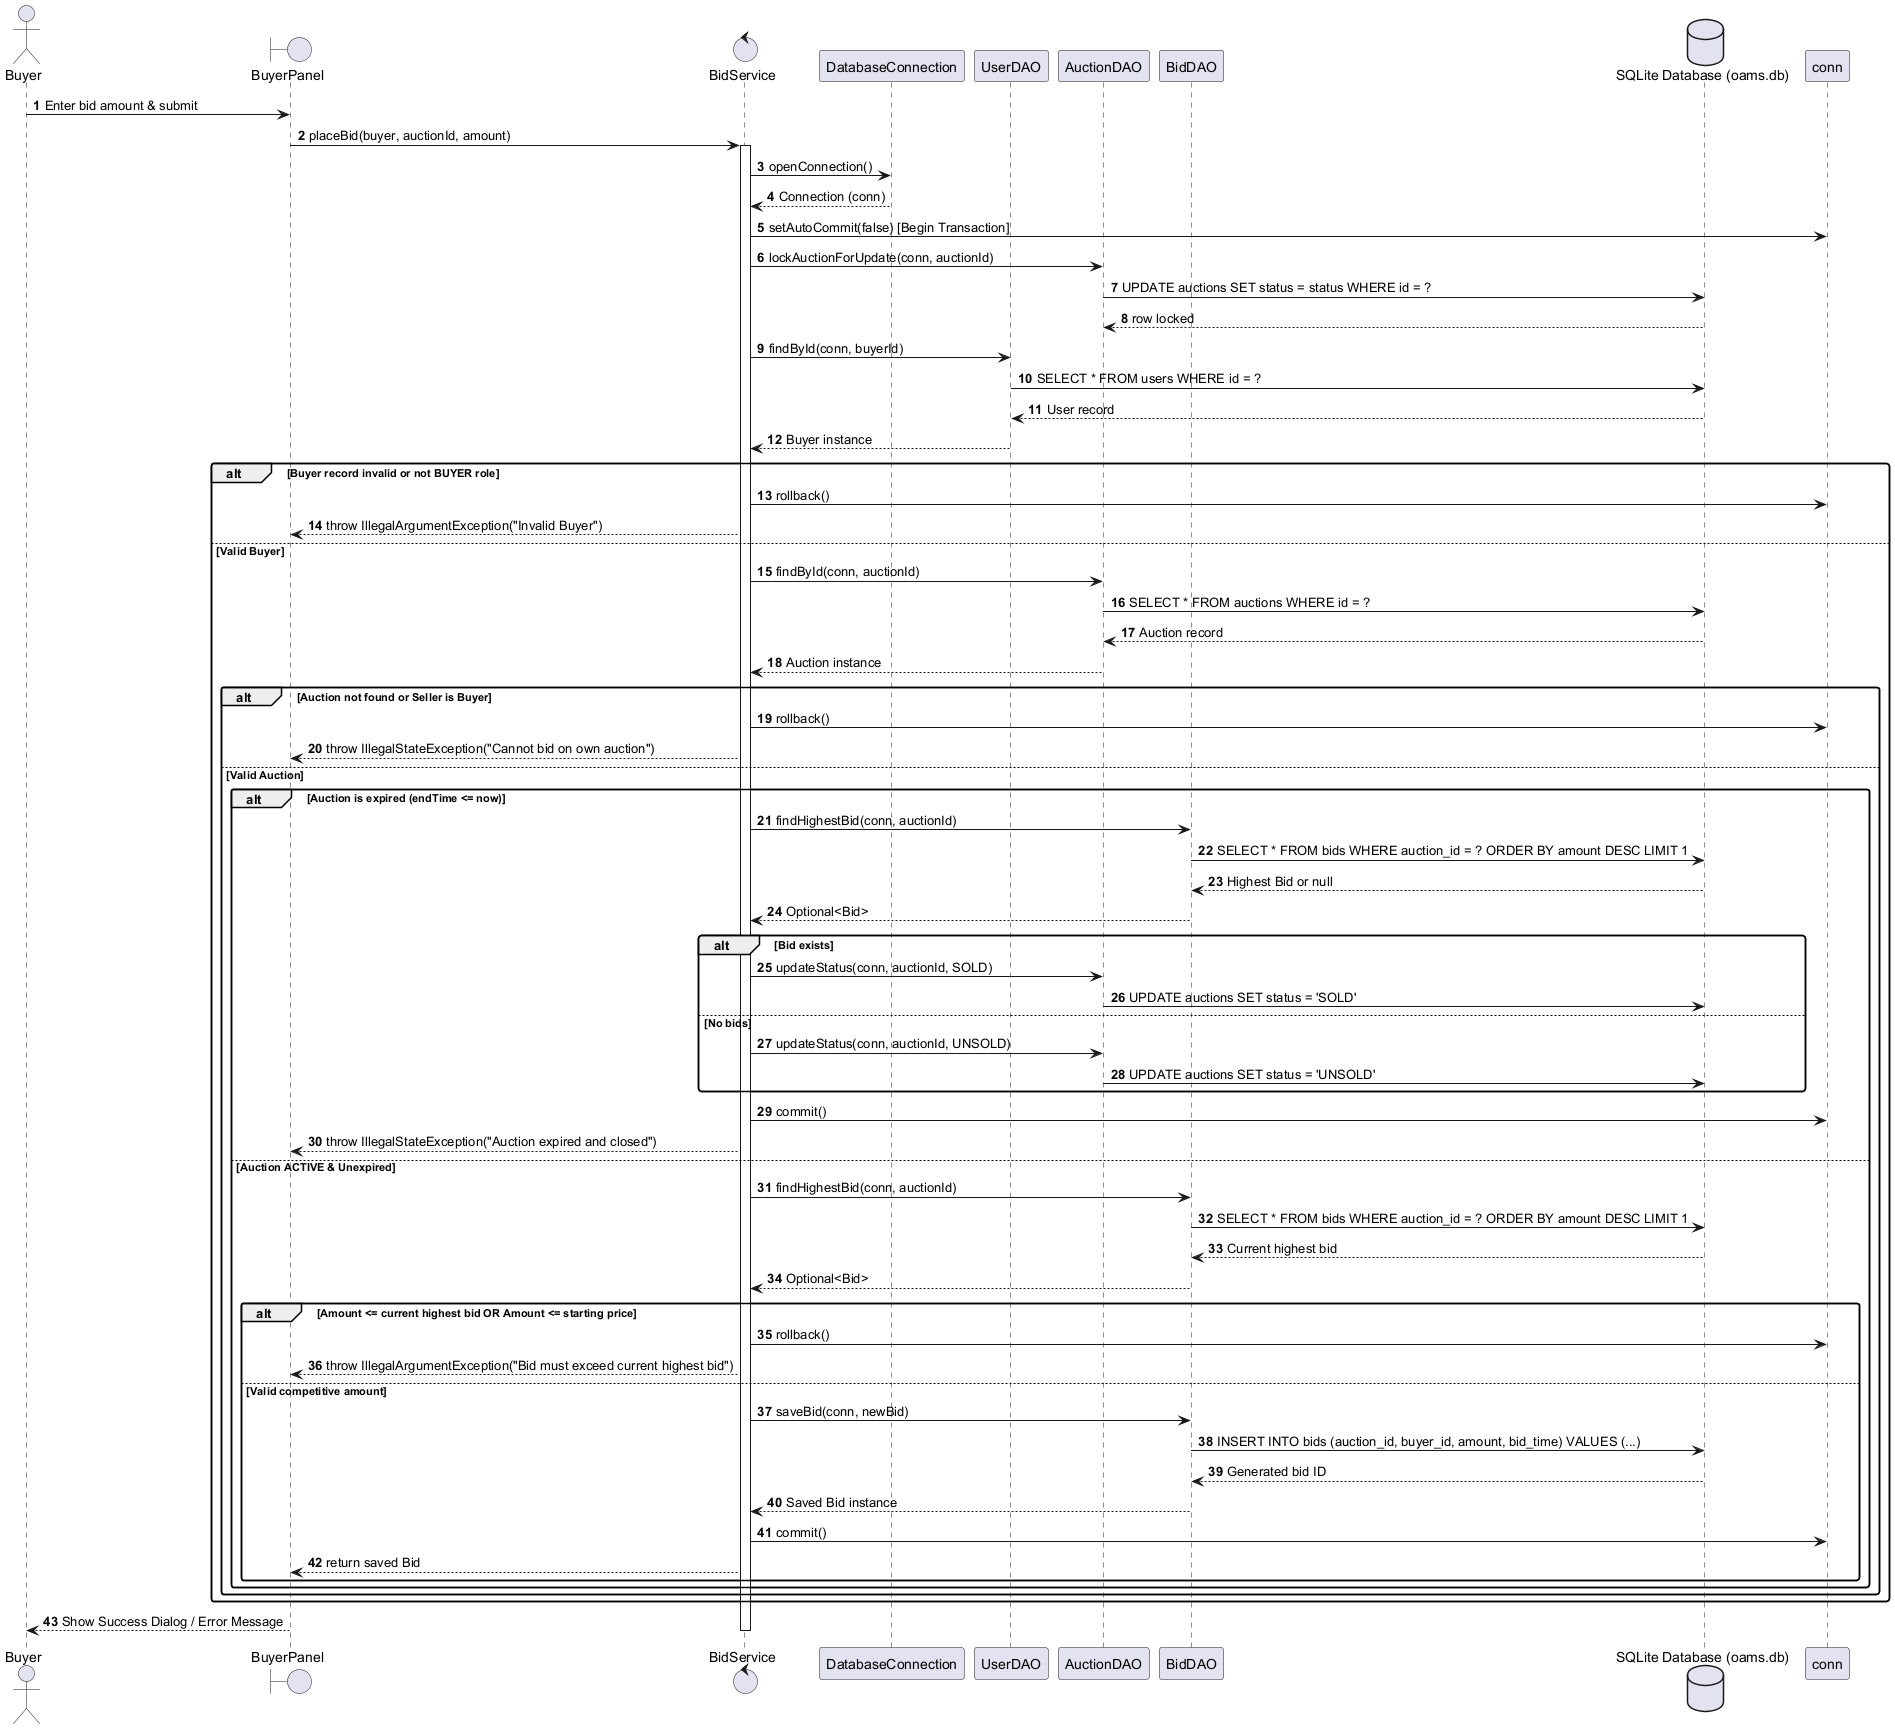
\includegraphics[width=0.98\textwidth]{figures/sequence_buyer_bid.png}
    \caption{UML Sequence Diagram: Transactional Bid Placement and Concurrency Locking}
    \label{fig:seq_bid}
\end{figure}

\paragraph{Step-by-Step Flow Analysis:}
\begin{enumerate}
    \item The Buyer inputs an amount in \texttt{BuyerPanel} and clicks ``Submit Bid''.
    \item \texttt{BuyerPanel} delegates to \texttt{BidService.placeBid(buyer, auctionId, amount)}.
    \item \texttt{BidService} obtains a JDBC connection and disables auto-commit (\texttt{setAutoCommit(false)}) to begin an ACID transaction.
    \item \texttt{BidService} calls \texttt{AuctionDAO.lockAuctionForUpdate(conn, auctionId)}, which issues a dummy update statement to acquire SQLite's reserved row/table lock.
    \item The buyer's persisted record is queried via \texttt{UserDAO.findById(conn, buyerId)} to verify that the buyer account exists and possesses the \texttt{BUYER} role. If invalid, the transaction rolls back.
    \item The target auction is fetched via \texttt{AuctionDAO.findById(conn, auctionId)}.
    \item \texttt{BidService} validates business rules:
    \begin{itemize}
        \item If the buyer is also the seller (\texttt{auction.getSellerId() == buyer.getId()}), the transaction is rolled back with an \texttt{IllegalStateException}.
        \item If the auction has expired (\texttt{now >= endTime}), \texttt{BidService} checks for existing bids. If present, status is updated to \texttt{SOLD}; otherwise, to \texttt{UNSOLD}. The transaction commits the status change, and the bid is rejected.
        \item If the auction is active and valid, \texttt{BidDAO.findHighestBid(conn, auctionId)} retrieves the current highest bid. If the submitted amount is less than or equal to the highest bid (or starting price), the transaction rolls back.
    \end{itemize}
    \item If all invariants pass, \texttt{BidDAO.saveBid(conn, bid)} inserts the new bid row.
    \item \texttt{BidService} commits the transaction (\texttt{conn.commit()}) and returns the persisted \texttt{Bid} object.
    \item \texttt{BuyerPanel} displays a success notification and refreshes bidding tables.
\end{enumerate}

\subsubsection{Scenario B: User Registration and Authentication}
Figure \ref{fig:seq_auth} illustrates user onboarding and authentication flows.

\begin{figure}[H]
    \centering
    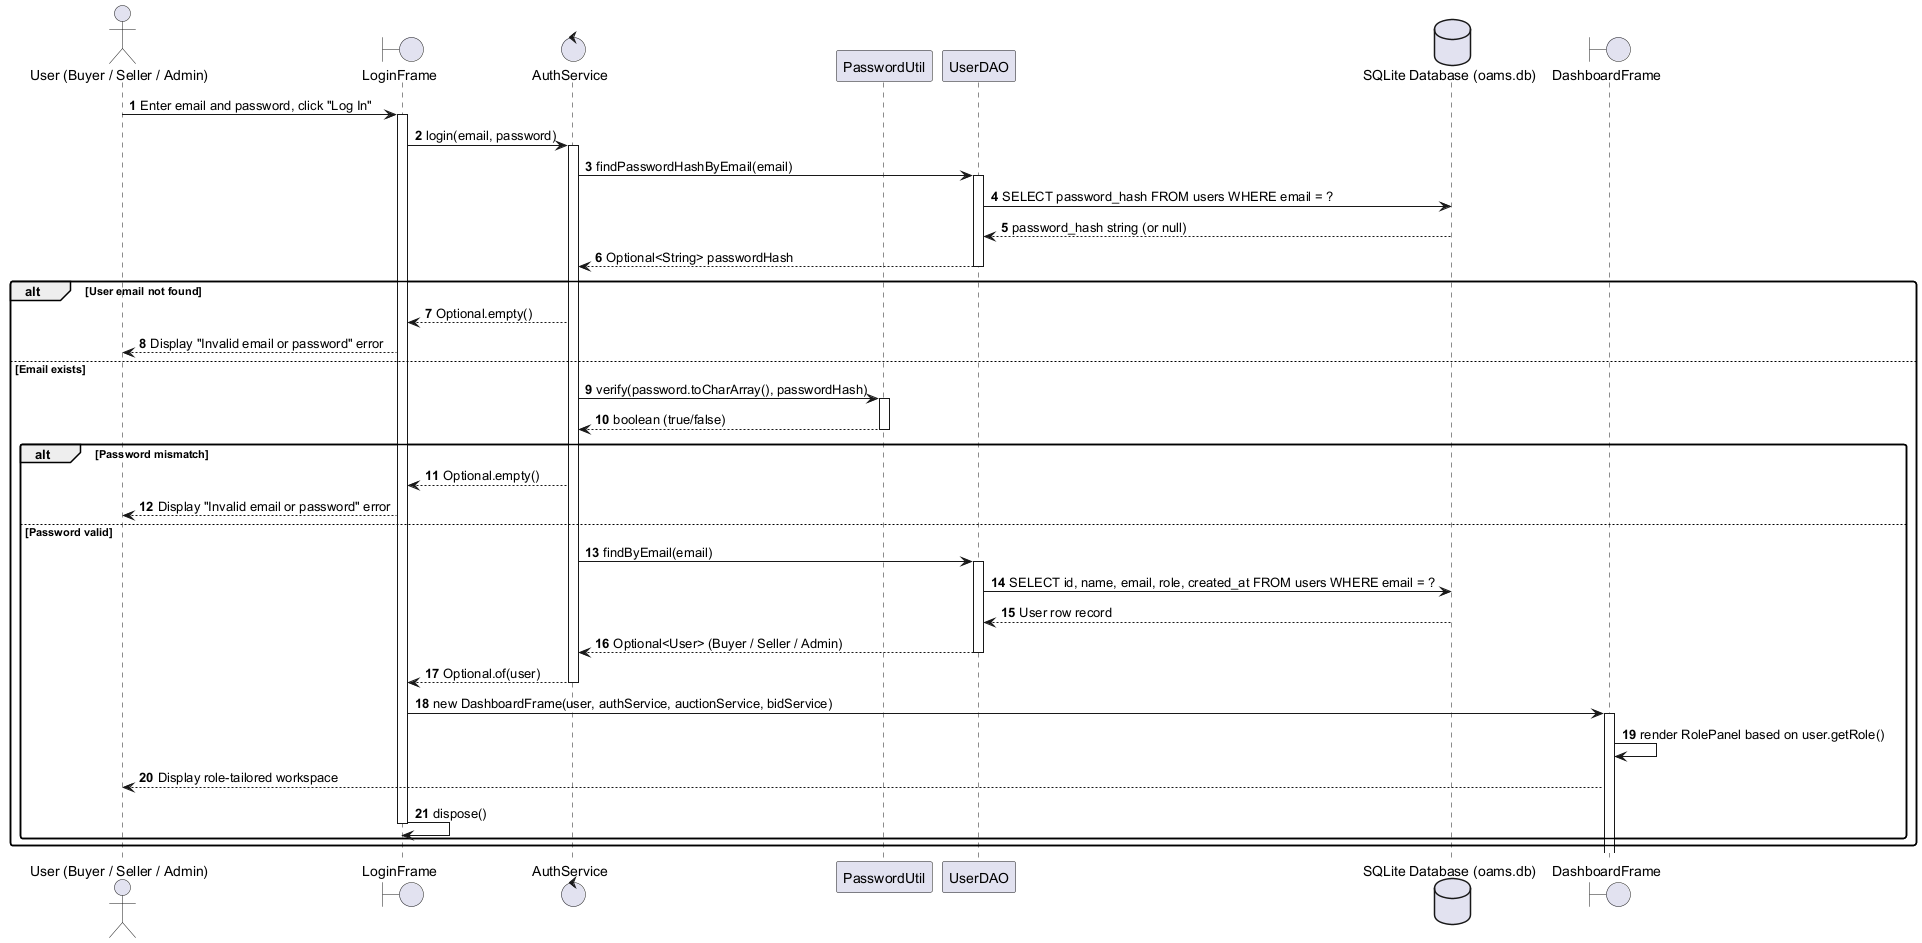
\includegraphics[width=0.95\textwidth]{figures/sequence_user_auth.png}
    \caption{UML Sequence Diagram: User Authentication and Dynamic Dashboard Initialization}
    \label{fig:seq_auth}
\end{figure}

\paragraph{Flow Analysis:}
The user enters credentials into \texttt{LoginFrame}, which forwards the request to \texttt{AuthService.login(email, password)}. The service queries \texttt{UserDAO.findPasswordHashByEmail(email)}. If a record exists, \texttt{PasswordUtil.verify(...)} evaluates the entered password against the stored PBKDF2 hash and salt. Upon verification, the user object is constructed from database fields and returned to \texttt{LoginFrame}, which disposes of itself and instantiates \texttt{DashboardFrame(user, ...)}. The dashboard inspects \texttt{user.getRole()} to render the appropriate workspace panel.

\subsubsection{Scenario C: Seller Creating an Auction}
Figure \ref{fig:seq_create} outlines the auction listing workflow.

\begin{figure}[H]
    \centering
    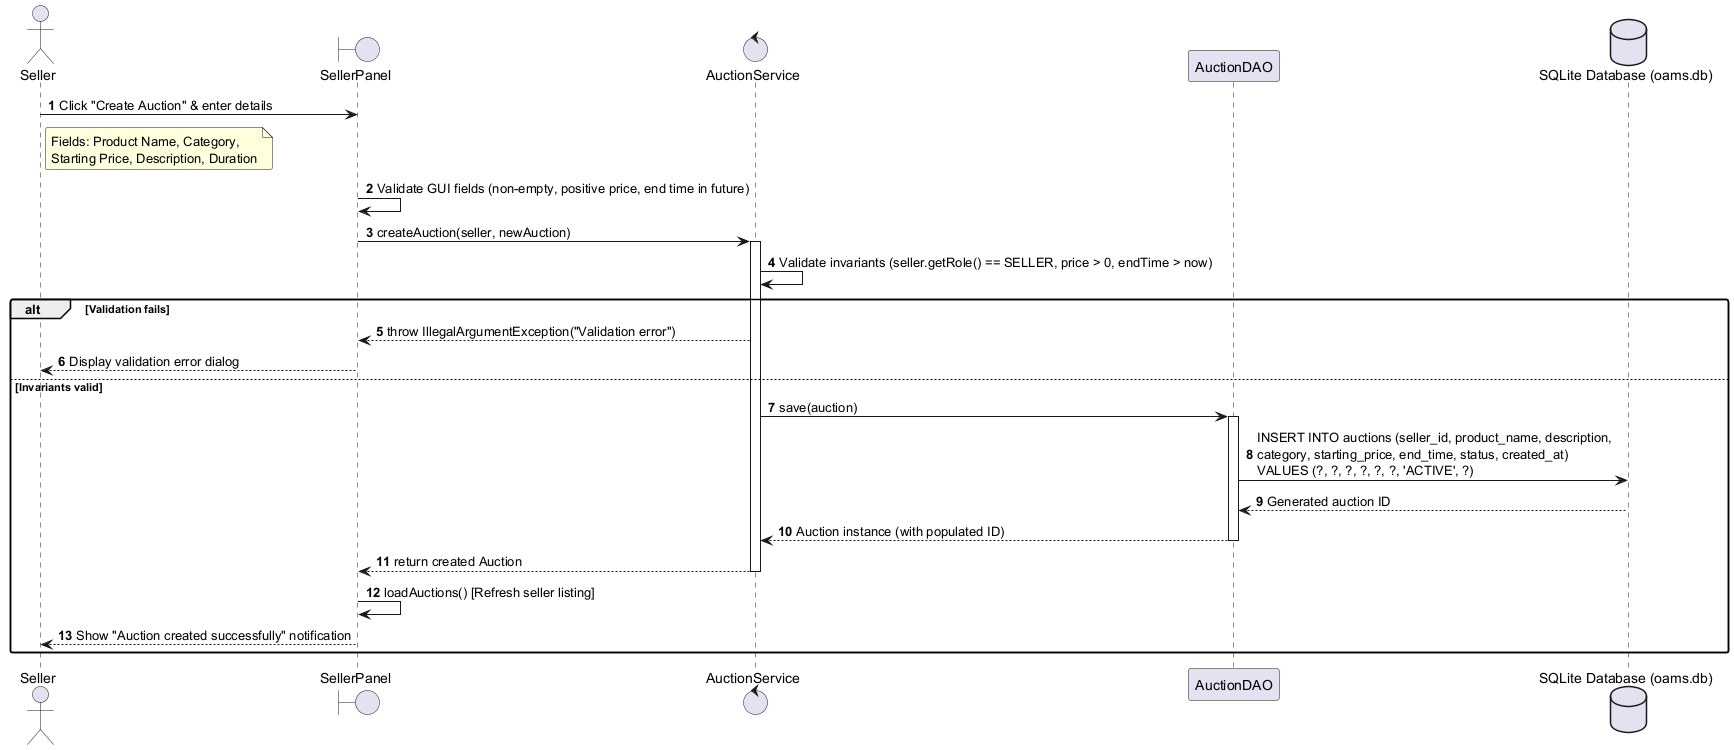
\includegraphics[width=0.90\textwidth]{figures/sequence_auction_create.png}
    \caption{UML Sequence Diagram: Seller Auction Listing Creation}
    \label{fig:seq_create}
\end{figure}

\paragraph{Flow Analysis:}
A Seller enters item details, starting price, and duration in \texttt{SellerPanel}. The panel constructs an \texttt{Auction} object, which enforces constructor validation (positive starting price, non-blank title). The panel calls \texttt{AuctionService.createAuction(seller, auction)}. The service verifies seller authorization, stamps the listing with \texttt{ACTIVE} status and creation timestamps, and delegates persistence to \texttt{AuctionDAO.save(auction)}. Upon successful insertion, the newly generated auction ID is returned, and the seller table refreshes automatically.

\subsubsection{Scenario D: Auction Closing and Winner Determination}
Figure \ref{fig:seq_close} depicts the automated lifecycle evaluation mechanism.

\begin{figure}[H]
    \centering
    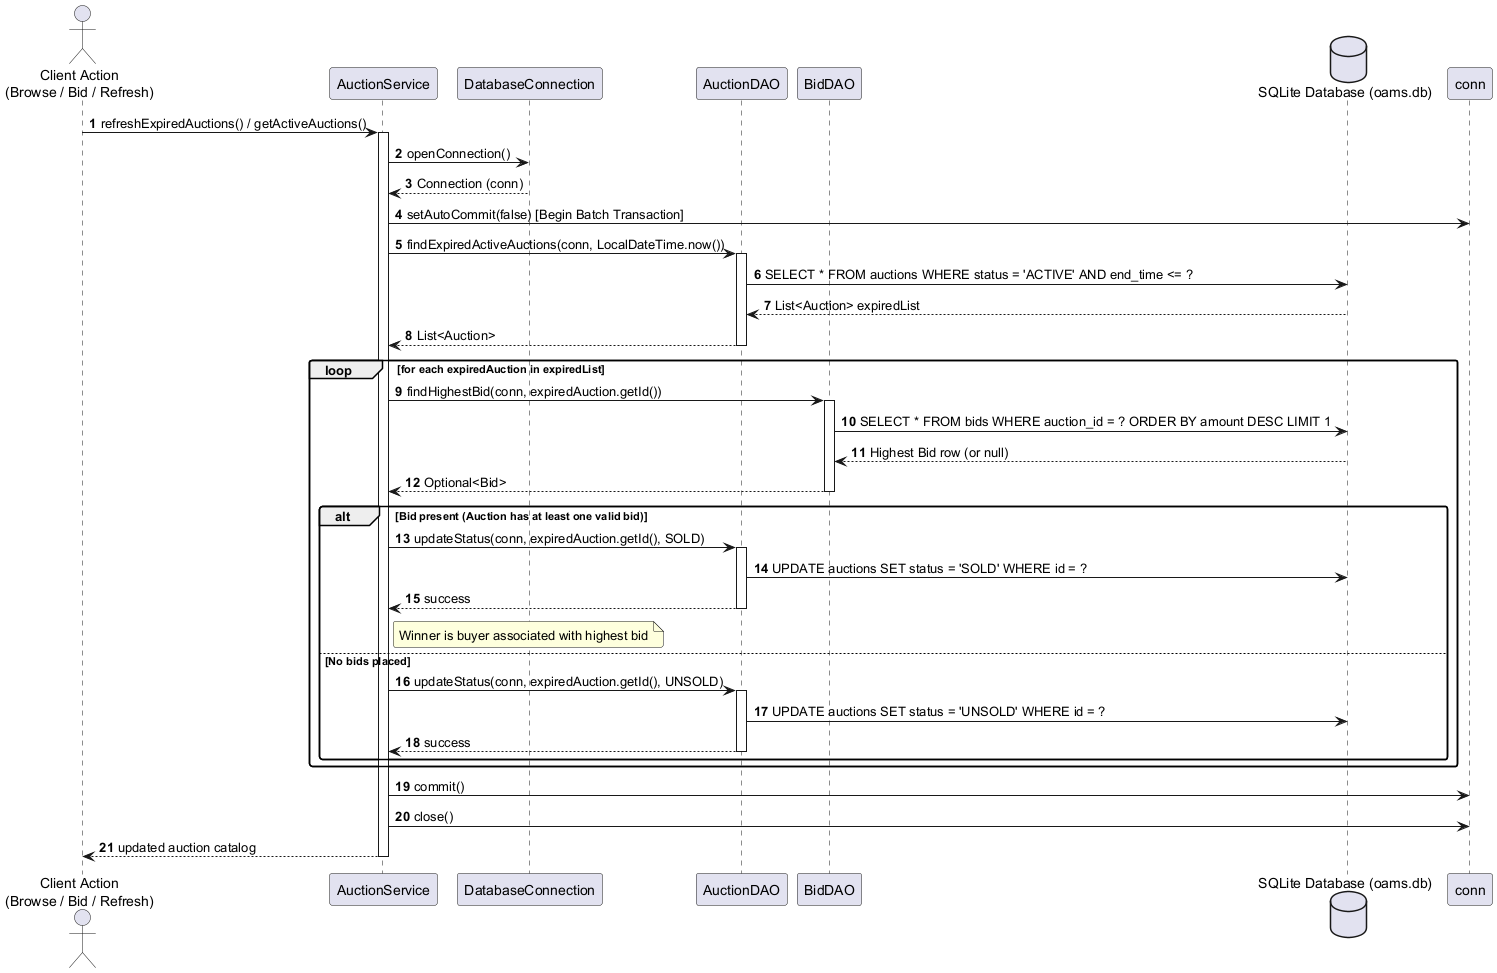
\includegraphics[width=0.95\textwidth]{figures/sequence_auction_close.png}
    \caption{UML Sequence Diagram: Lazy Auction Closing and Winner Settlement}
    \label{fig:seq_close}
\end{figure}

\paragraph{Flow Analysis:}
Auction settlement is evaluated on demand via a \textit{lazy expiration pattern}. Whenever an active catalog is requested or a bid is placed, \texttt{AuctionService.refreshExpiredAuctions()} executes. Within an ACID transaction, \texttt{AuctionDAO.findExpiredActiveAuctions(conn, now)} queries listings whose \texttt{end\_time} is in the past. For each expired listing:
\begin{itemize}
    \item If \texttt{BidDAO.findHighestBid(conn, auctionId)} returns a bid, the auction transitions to \texttt{SOLD}, establishing the highest bidder as the winner.
    \item If no bids exist, the auction transitions to \texttt{UNSOLD}.
\end{itemize}
The batch transaction is committed, ensuring catalog consistency without requiring an external scheduling process.

\subsubsection{Scenario E: Administrator Cancelling an Auction}
Figure \ref{fig:seq_cancel} models administrative listing moderation.

\begin{figure}[H]
    \centering
    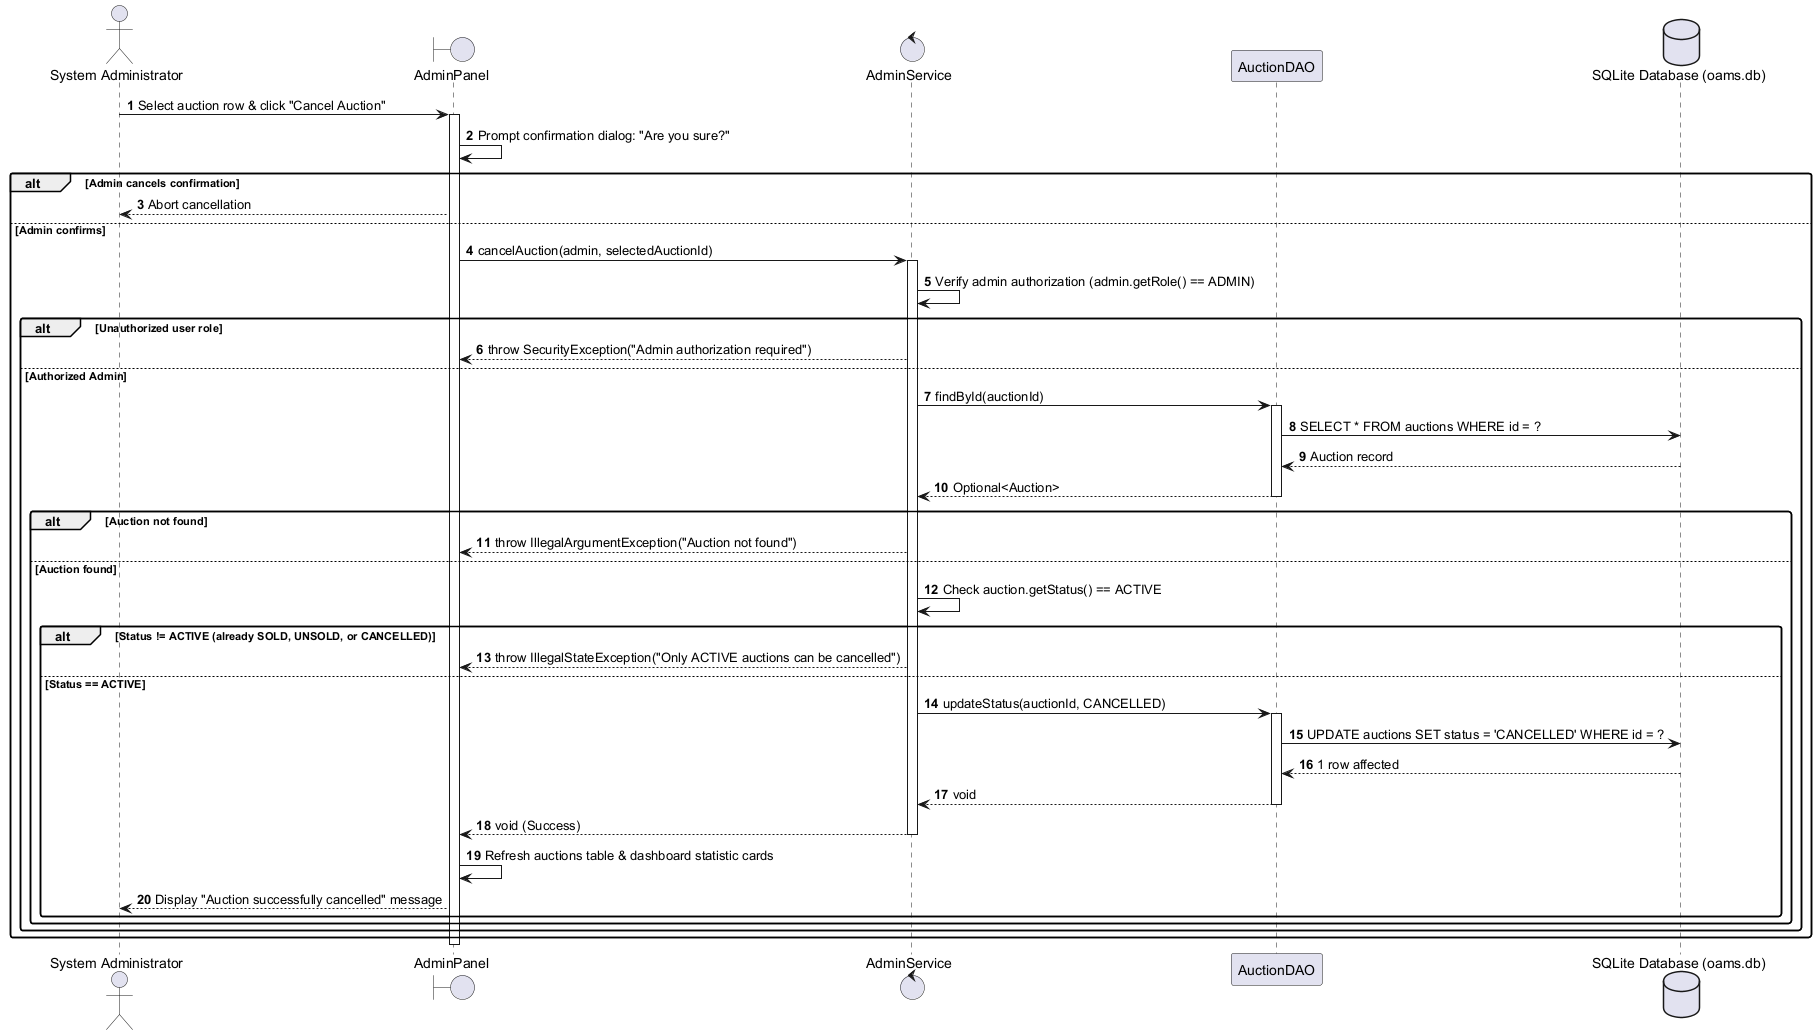
\includegraphics[width=0.95\textwidth]{figures/sequence_admin_cancel.png}
    \caption{UML Sequence Diagram: Administrative Auction Moderation and Cancellation}
    \label{fig:seq_cancel}
\end{figure}

\paragraph{Flow Analysis:}
An Administrator selects an auction in the Admin Panel and clicks ``Cancel Auction''. A confirmation dialog prompts for verification. Upon confirmation, \texttt{AdminService.cancelAuction(admin, auctionId)} is invoked. The service verifies that the invoking user possesses the \texttt{ADMIN} role and confirms via \texttt{AuctionDAO.findById(auctionId)} that the auction is currently in the \texttt{ACTIVE} state. If the auction is already \texttt{SOLD}, \texttt{UNSOLD}, or \texttt{CANCELLED}, the operation is rejected. Otherwise, \texttt{AuctionDAO.updateStatus(auctionId, CANCELLED)} updates the status. The Admin Panel then refreshes the auction table and updates dashboard metrics.

% ==============================================================================
% 4. ACTIVITY DIAGRAM
% ==============================================================================
\subsection{Activity Diagram (Workflow and Decision Logic)}
\label{subsec:uml_activity}

\subsubsection{Diagram Visualization}
Figure \ref{fig:activity_diagram} captures the end-to-end control flow of user interactions across different roles.

\begin{figure}[H]
    \centering
    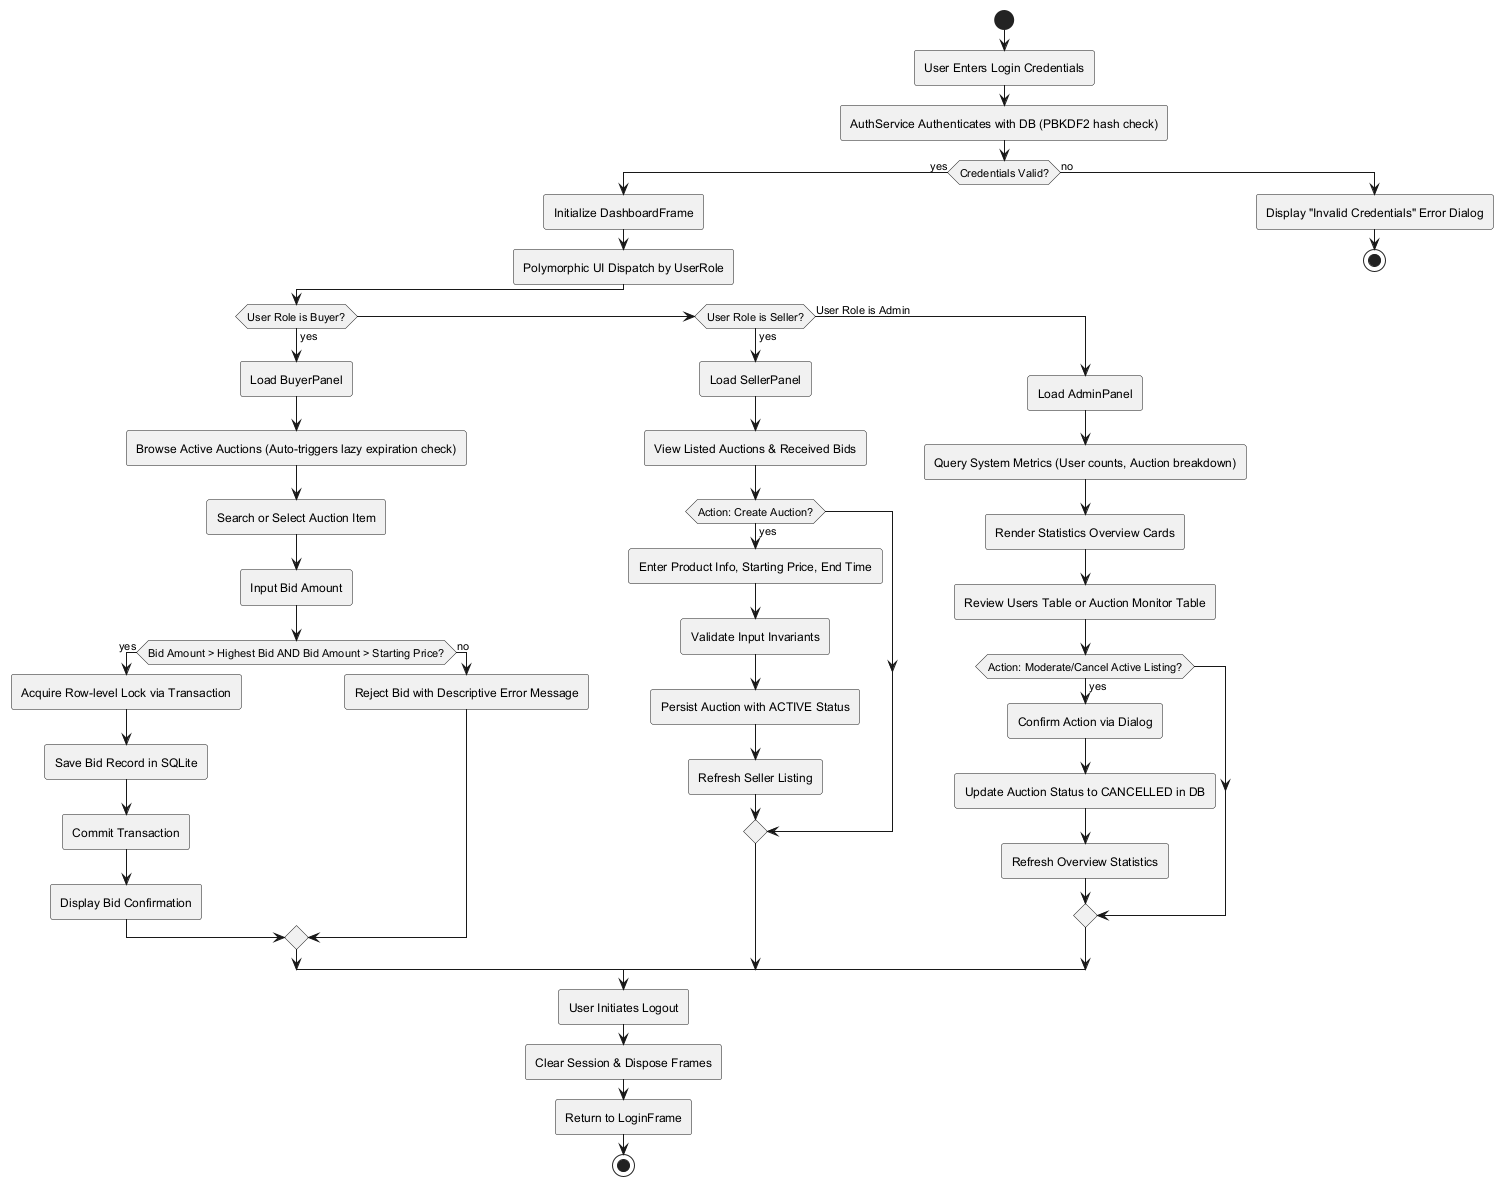
\includegraphics[width=0.85\textwidth]{figures/activity_diagram.png}
    \caption{UML Activity Diagram: End-to-End System Workflow and Decision Logic}
    \label{fig:activity_diagram}
\end{figure}

\subsubsection{Workflow Analysis}
The Activity diagram highlights conditional branching and concurrency controls:
\begin{enumerate}
    \item \textbf{Authentication Branching:} Credentials undergo hash validation. Failure routes to an error notification and halts the session; success branches into polymorphic role dashboards.
    \item \textbf{Buyer Bidding Path:} Includes active auction browsing, lazy expiration evaluation, bid amount comparison, transactional row locking, and database updates.
    \item \textbf{Seller Path:} Supports auction creation with invariant validation and tracking of received bids.
    \item \textbf{Admin Path:} Provides live metric queries, multi-criteria filtering, and listing moderation.
\end{enumerate}

% ==============================================================================
% 5. STATE MACHINE DIAGRAM
% ==============================================================================
\subsection{State Machine Diagram (Auction Entity Lifecycle)}
\label{subsec:uml_state_machine}

\subsubsection{Diagram Visualization}
Figure \ref{fig:state_machine} presents the finite state machine governing an \texttt{Auction} entity throughout its operational lifecycle.

\begin{figure}[H]
    \centering
    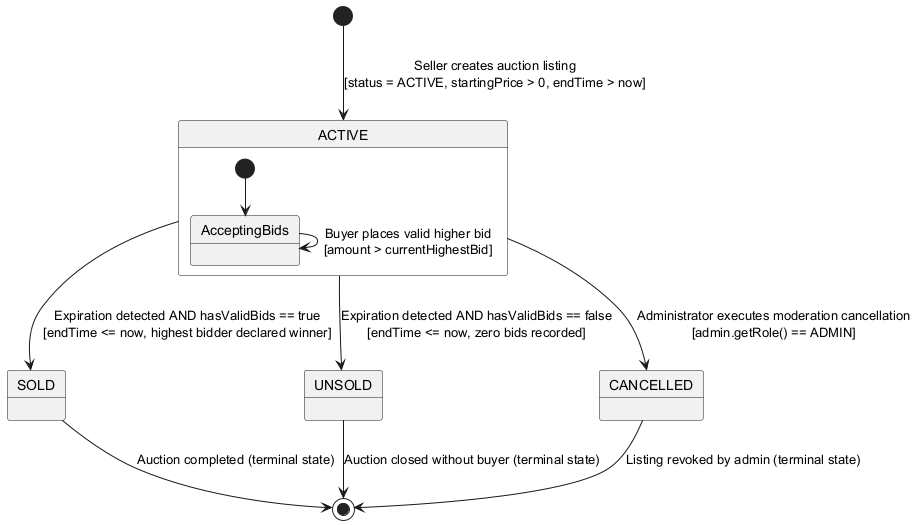
\includegraphics[width=0.85\textwidth]{figures/state_machine_diagram.png}
    \caption{UML State Machine Diagram for the \texttt{Auction} Entity}
    \label{fig:state_machine}
\end{figure}

\subsubsection{State Transitions and Guard Conditions}
An auction listing transitions through well-defined lifecycle states:
\begin{itemize}
    \item \textbf{Initial State $\rightarrow$ \texttt{ACTIVE}:} Transition occurs upon valid auction creation by an authenticated Seller with positive starting price and future end time.
    \item \textbf{\texttt{ACTIVE} Internal State (Accepting Bids):} While in \texttt{ACTIVE}, the auction receives bids. Each valid bid updates the prevailing highest price.
    \item \textbf{\texttt{ACTIVE} $\rightarrow$ \texttt{SOLD}:} Triggered when \texttt{now $\ge$ endTime} and \texttt{hasValidBids == true}. The highest bidder is declared the winner.
    \item \textbf{\texttt{ACTIVE} $\rightarrow$ \texttt{UNSOLD}:} Triggered when \texttt{now $\ge$ endTime} and \texttt{hasValidBids == false}. The listing terminates without sale.
    \item \textbf{\texttt{ACTIVE} $\rightarrow$ \texttt{CANCELLED}:} Triggered when an Administrator moderates an active listing.
    \item \textbf{Terminal States:} \texttt{SOLD}, \texttt{UNSOLD}, and \texttt{CANCELLED} are terminal states; no further transitions or bid submissions are permitted.
\end{itemize}

% ==============================================================================
% 6. COMPONENT DIAGRAM
% ==============================================================================
\subsection{Component Diagram (Structural Decomposition)}
\label{subsec:uml_component}

\subsubsection{Diagram Visualization}
Figure \ref{fig:component_diagram} models the modular software components and their interface dependencies.

\begin{figure}[H]
    \centering
    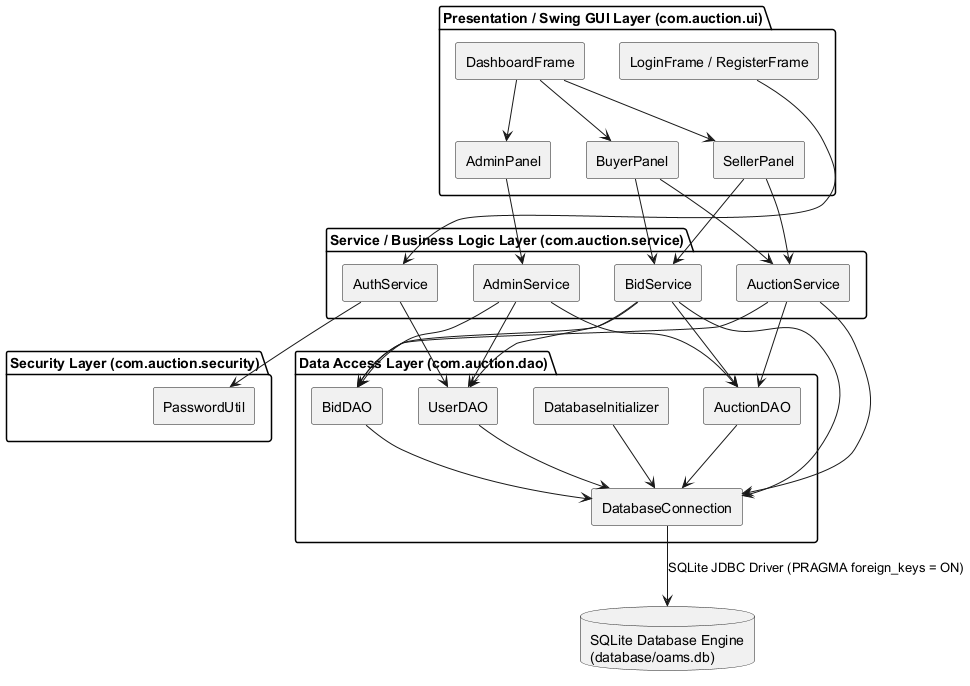
\includegraphics[width=0.92\textwidth]{figures/component_diagram.png}
    \caption{UML Component Diagram: Architectural Tiers and Inter-Component Dependencies}
    \label{fig:component_diagram}
\end{figure}

\subsubsection{Component Architecture}
The software is organized into four distinct architectural layers:
\begin{itemize}
    \item \textbf{Presentation Component:} Houses Swing frames and panels (\texttt{LoginFrame}, \texttt{DashboardFrame}, \texttt{BuyerPanel}, \texttt{SellerPanel}, \texttt{AdminPanel}).
    \item \textbf{Service Component:} Encapsulates business logic and orchestration (\texttt{AuthService}, \texttt{AuctionService}, \texttt{BidService}, \texttt{AdminService}).
    \item \textbf{Security Component:} Isolates cryptographic routines (\texttt{PasswordUtil}).
    \item \textbf{Data Access Component:} Encapsulates persistence logic and JDBC interactions (\texttt{UserDAO}, \texttt{AuctionDAO}, \texttt{BidDAO}, \texttt{DatabaseConnection}).
\end{itemize}

% ==============================================================================
% 7. DEPLOYMENT DIAGRAM
% ==============================================================================
\subsection{Deployment Diagram (Hardware and Runtime Environment)}
\label{subsec:uml_deployment}

\subsubsection{Diagram Visualization}
Figure \ref{fig:deployment_diagram} details the physical runtime environment and artifact deployment.

\begin{figure}[H]
    \centering
    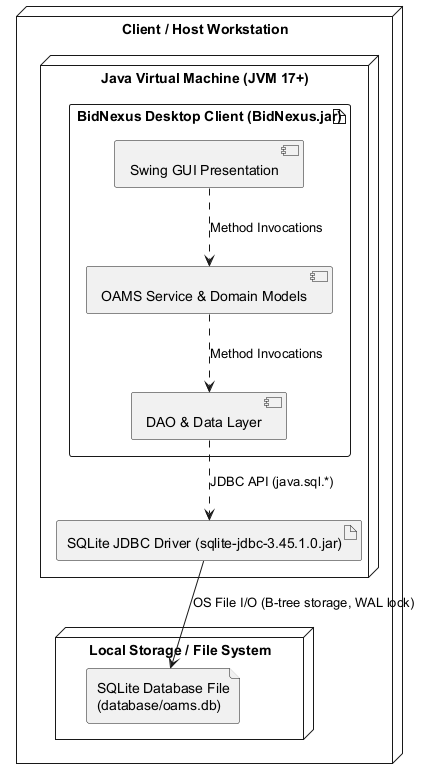
\includegraphics[width=0.85\textwidth]{figures/deployment_diagram.png}
    \caption{UML Deployment Diagram: Client Workstation Runtime Environment}
    \label{fig:deployment_diagram}
\end{figure}

\subsubsection{Deployment Architecture}
The system deploys as a standalone desktop application on a client workstation:
\begin{itemize}
    \item \textbf{Host Machine:} Any modern operating system (Windows, Linux, macOS) equipped with a Java Virtual Machine (JVM, JDK 17+).
    \item \textbf{Application Artifact:} The executable JAR file (\texttt{BidNexus.jar}), packaging presentation, service, and data access components.
    \item \textbf{Database Driver:} The SQLite JDBC Driver library (\texttt{sqlite-jdbc-3.45.1.0.jar}) embedded within the classpath.
    \item \textbf{Database Storage:} A local database file (\texttt{database/oams.db}), managed through filesystem file I/O with ACID transactional semantics.
\end{itemize}

% ==============================================================================
% 8. ENTITY-RELATIONSHIP (ER) DIAGRAM
% ==============================================================================
\subsection{Entity-Relationship (ER) Diagram (Relational Data Model)}
\label{subsec:uml_er}

\subsubsection{Diagram Visualization}
Figure \ref{fig:er_diagram} presents the Entity-Relationship model corresponding to the SQLite relational schema.

\begin{figure}[H]
    \centering
    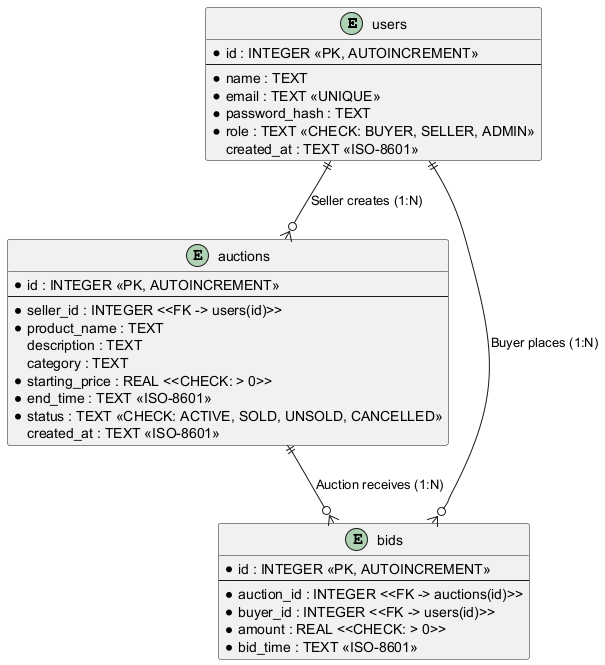
\includegraphics[width=0.88\textwidth]{figures/er_diagram.png}
    \caption{Entity-Relationship (ER) Diagram of the SQLite Relational Schema}
    \label{fig:er_diagram}
\end{figure}

\subsubsection{Entities, Attributes, and Cardinalities}
The database schema consists of three core relational tables:
\begin{itemize}
    \item \textbf{\texttt{users} Entity:} Stores user profiles. Attributes include \texttt{id} (PK), \texttt{name}, \texttt{email} (Unique), \texttt{password\_hash}, \texttt{role} (CHECK constraint), and \texttt{created\_at}.
    \item \textbf{\texttt{auctions} Entity:} Stores auction listings. Attributes include \texttt{id} (PK), \texttt{seller\_id} (FK referencing \texttt{users.id}), \texttt{product\_name}, \texttt{description}, \texttt{category}, \texttt{starting\_price} (CHECK $> 0$), \texttt{end\_time}, \texttt{status} (CHECK constraint), and \texttt{created\_at}.
    \item \textbf{\texttt{bids} Entity:} Stores bid transactions. Attributes include \texttt{id} (PK), \texttt{auction\_id} (FK referencing \texttt{auctions.id}), \texttt{buyer\_id} (FK referencing \texttt{users.id}), \texttt{amount} (CHECK $> 0$), and \texttt{bid\_time}.
    \item \textbf{Cardinalities:}
    \begin{itemize}
        \item One Seller can create zero or more Auctions ($1:N$).
        \item One Auction can receive zero or more Bids ($1:N$).
        \item One Buyer can place zero or more Bids ($1:N$).
    \end{itemize}
\end{itemize}
All foreign keys are strictly enforced at runtime via SQLite's foreign key pragma.
